\documentclass{article}

\usepackage{dirtree}
\usepackage[dvipsnames]{xcolor}
\usepackage{amssymb}
\usepackage{amsmath}
\usepackage{algpseudocode}
\usepackage{algorithm}
\usepackage{todonotes}
\usepackage{hyperref}
\usepackage{multirow}
\usepackage{biblatex}
\addbibresource{references.bib}
\usepackage{tcolorbox}
\newtcolorbox{invariant}[1][]{%
   attach title to upper={\ },
   title=#1,
}

% Source - https://tex.stackexchange.com/a/306992
% Posted by egreg
% Retrieved 2026-06-25, License - CC BY-SA 3.0
\makeatletter
\pdfstringdefDisableCommands{\let\(\fake@math}
\newcommand\fake@math{}% just for safety
\def\fake@math#1\){[math]}
\makeatother


\title{Optimization of Invariant Verification for Safe Replication of BFT-Logs}
\author{Pascal von Fellenberg}
\begin{document}
\maketitle
%\newcommand{\todo}[1]{\emph{\colorbox{Yellow}{TODO #1}}}
\newcommand{\balance}[0]{\textsc{Balance}}
\newcommand{\apply}[0]{\textit{apply}}
\newcommand{\acc}[0]{\textit{acc}}
\newcommand{\msgId}[0]{\texttt{MsgId}}
\newcommand{\deltacc}[1]{#1^\delta}
\newcommand{\var}[1]{\textsl{#1}}
\newcommand{\msgType}[0]{\texttt{MsgType}}
\newcommand{\forkproof}[0]{\var{forkProof}}
\newcommand{\definedas}[0]{\stackrel{def}{=}}
\setlength{\marginparwidth}{100pt}

\section*{Abstract}
TODO
\section*{Acknowledgements}
TODO

\tableofcontents

\section{Introduction}
Contributions:
\begin{enumerate}
    \item algorithm for verifying GOC-Ledger state.
    \item efficient encoding of delta account as commit messages.
    \item proposal of new message type (byzantine acknowledgement)
    \item invariants $\delta1$ to $\delta8$ and $F1$ to $F3$
\end{enumerate}
TODO

\section{Background}
In this section, relevant background to the concepts in this project are provided. \\

\subsection{Append-only logs as Hash-Graphs}
An Append-only log is a distributed data structure that allows participants to share messages between each other. This is done by having each participant have a totally ordered set of messages that gets replicated to the other participants. This can be implemented using hash-graphs, where each message contains the hash of the previous message (if there is any) of the same author. By using a cryptographic hash, we know the messages cannot have been tampered with, as hash-collisions are computationally hard to find. By cryptographically signing the messages we can guarantee that the correct author created the message.

However one problem that arises is that an adversary E can create two messages that are concurrent to each other by referencing the same previous message and distributing each of those messages to different parts of the network. Once the correct participants have replicated these messages, this results in the set of messages belonging to E no longer being totally ordered, breaking the design of naive implementations of append-only logs. In this scenario we say that the log of E is \emph{forked} and E is an \emph{equivocator} \cite{blocklace-crdt}.

If the append-only log is implemented as a hash-graph, dependencies between messages of different authors can be modelled by including a set of hashes into a message which represent its immediate dependencies. Such dependencies are necessary to order messages by causality, i.e. if there is a hash in the dependencies of message A belonging to message B, we know the message B must have been created before the message A (see happens-before relationship, eqn. \ref{eqn:happens-before}).

\subsection{2P-BFT-Log}
2P-BFT-Log is a design that implements an append-only log data structure and behaves just like one as long as there are no forks. As soon as there is evidence of a fork in a log, any further messages of the corresponding author are ignored \cite{2p-bft-log}. If there is no fork in a given log, the log is said to be in the \emph{growing phase}, otherwise it is in the \emph{shrinking phase}.

\subsubsection{Messages}
The design of 2P-BFT-Log consists of several parts. First of all, each message has certain contents, each of which is called a field. The fields of a message and their corresponding type and meaning are listed in Table \ref{tab:2p-bft-log-msg-content}.

\begin{table}
    \begin{tabular}{|l|l|p{5cm}|}
    \hline
    \textbf{Field} & \textbf{Type} & \textbf{Meaning}\\
    \hline
    $M_\emph{author}$ & String (Public Key) & author of the message \\
    $M_\emph{prev}$ & MsgId or $\bot$ & previous message from same author, $\bot$ (null) if none.\\
    $M_\emph{deps}$ & Set of MsgId & State of logs from other authors on which the message depends\\
    $M_\emph{payload}$ & String & Content of message, in our case representing either an account update or a byzantine acknowledgement (see sections \ref{sec:account-as-str} and \ref{sec:ack-as-str} respectively) \\
    $M_\emph{signature}$ & String & Signature of the concatenation of the previous fields using the private key corresponding to $M_\emph{author}$.\\
    \hline
    \end{tabular}
    \caption{Contents of a message according to the design of 2P-BFT-Log}
    \label{tab:2p-bft-log-msg-content}
\end{table}

To identify and reference messages, the function $\msgId$ is used.
It is the hash derived from the concatenation of the contents of the message, i.e.
\[
    \msgId(M) \definedas H(M_\emph{author} \oplus M_\emph{prev} \oplus M_\emph{deps} \oplus M_\emph{payload} \oplus M_\emph{signature})
\]
where $H$ is a cryptographic hash function.

Additionally there are some relevant relations that are defined on messages.
The first one is the \emph{happens-before} relationship and is defined as:
\begin{equation}
    M \rightsquigarrow M' \definedas \begin{cases}
        M = M'_\emph{prev} = \bot \\
        \msgId(M) = M'\emph{prev} \\
        \msgId(M) \in M'\emph{deps} \\
        \exists M'' : M \rightsquigarrow M'' \rightsquigarrow M'
    \end{cases}
    \label{eqn:happens-before}
\end{equation}

Based on the happens-before relationship, the partial order on messages ($\le_\mathcal{M}$) is defined:\todo{is this relevant for my report?}
\[
    M \le_\mathcal{M} M' \definedas M = M' \lor M \rightsquigarrow M'
\]

If neither $M$ or $M'$ is smaller than the other, they are called concurrent ($\parallel_\mathcal{M}$). \todo{is this relevant for my report?}
\[
    M \parallel_\mathcal{M} M' \definedas M {\nleq_\mathcal{M}} M' \land M' {\nleq_\mathcal{M}} M
\]

We define the strict causal history of message $M$ as the messages that happened before message $M$:
\[
    \mathcal H_<(M) \definedas \{M' : M' \rightsquigarrow M\}
\]
Additionally we define the causal history of message $M$ as
\[
    \mathcal H_\le(M) \definedas \{M' : M' \le_\mathcal{M} M\}
\]

If $S$ is a set of messages, the (strict) causal history of $S$ is overloaded and means the (strict) causal history of all the messages in $S$ combined.
\[
    \mathcal H_r(S) \definedas \bigcup_{M \in S}\mathcal H_r(M)
\]


\subsubsection{Logs}
A log in the context of 2P-BFT-Log is defined as a datastructure that keeps track of the state of the application. Log $L$ has the fields $L_\emph{author}$, $L_\emph{last}$ which contains the last message of this author and $L_\emph{forks}$ which contains the oldest known fork proof of this author. \todo{if necessary add more description here}

\subsubsection{Frontier}
TODO

\subsection{\(\delta\)-GOC-Ledger}

The Grow-Only-Counter-Ledger (GOC-Ledger) is a consensus-free data structure that implements a ledger designed to be used to track transactions of crypto-tokens. A ledger needs to track which author owns how many tokens, to be able to check how many tokens they are able to spend in subsequent transactions. An account $A$ is the unit of data that keeps track of this information. Multiple such accounts from different authors of the state of the ledger. More concretely, a ledger $L$ is a mapping from authors to their corresponding account.

In the case of the GOC-Ledger, this is realized by introducing 5 fields: $A_\emph{author}$ which is the author of this account, $A_\uparrow$ and $A_\downarrow$ which represent the number of created/destroyed tokens respectively, $A_\rightarrow$ and $A_\leftarrow$ which represent the number of given/received tokens respectively. $A_\uparrow$ and $A_\downarrow$ are simple grow-only counters whereas $A_\rightarrow$ and $A_\leftarrow$ are mappings from author names to grow-only counters, which represent the number of tokens $A_\emph{author}$ has given to or acknowledged from the other author respectively.

For ease of writing, the notation $S_*$ is defined to be the domain of definition of a mapping $S$. E.g. if $L$ is a ledger, $L_*$ denotes the set of authors that have an account in this ledger. \todo{where should I put this definition?}

To get the balance of an account, we can compute \[\balance(A) \definedas A_\uparrow + \left(\sum_{a \in A_{\leftarrow*}} A_\leftarrow[a]\right) - A_\downarrow - \left(\sum_{a \in A_{\rightarrow*}} A_\rightarrow[a]\right)\].
Additionally there is a merge operation with which accounts can be merged. This merge function is only defined on accounts of the same author and returns the account that contains the maximal values of all the grow only counters in both of the accounts and adds all the grow-only counters that are only in one of the two accounts. \todo{write down the definition of this merge operation}

Furthermore, there is also a merge operation on the ledger and a delta account. The ledger and a delta-account get merged by merging the account with the corresponding account in the ledger if the author is present and if not, adding the account to the ledger. \todo{define this more precisely if necessary?}

The merge operation between two objects is denoted $\sqcup$.

\subsubsection{Delta Accounts}
To store the state of the ledger more efficiently with regards to space, only the grow-only counters that have changed have to be stored. This is done via delta accounts as proposed by Heisch \cite{delta-goc-ledger-heisch}. A delta account $A^\delta$ has the same fields as a normal account, just that the fields $A^\delta_\uparrow$ and $A^\delta_\downarrow$ can have a null value (denoted $\bot$) which represents a missing value. Such a null value is not needed for $A^\delta_\rightarrow$ and $A^\delta_\leftarrow$ because the empty set is a natural empty value. When merging delta accounts, one can use a slightly modified version of the merge operation on normal accounts, one just has to treat $\bot$ as a 0.


\section{Design}

\subsection{Definitions}
\todo{add description of the used notation here}
\todo{introduce induced frontier}

$\textsc{CheckSignature}$ of message $M$ is the predicate that is true iff $M_\emph{signature}$ is a valid signature belonging to $M_\emph{author}$.

A fork proof is a set of messages which all have the same previous message. We define fork proofs as a predicate $\forkproof$ over a set of messages $S$.
\begin{multline*}
    \forkproof(S) \definedas \\
    \hfill\bigwedge_{M, M' \in S} \left(
        \begin{aligned}
            &M_\emph{prev} = M'_\emph{prev}
            \land M_\emph{author} = M'_\emph{author} \\
            &\land \textsc{CheckSignature}(M)
            \land \textsc{CheckSignature}(M')
        \end{aligned}
    \right)
\end{multline*}

The function \var{deps} of message $M$ is defined as the messages in its immediate dependencies.
\[\var{deps}(M) \definedas \{M' \mid \msgId(M') \in M_\emph{deps}\}\]

Similarly, the function \var{prev} of $M$ denotes its previous message.
\[\var{prev}(M) \definedas \begin{cases}
    M' &\text{ if there exists } M' : \msgId(M') = M_\emph{prev}\\
    \bot & \text{ otherwise}
\end{cases} \]

A message $M$ in our design can have one of two types; either it has the type account (denoted \var{ACCOUNT}) or it has the type byzantine acknowledgement (denoted \var{BYZ\_ACK}). The type is encoded within its payload and retrieved with $\msgType(M)$. The roles of these message types is specified in \ref{sec:choices}. The function $\acc$ is the function that retrieves the account fields encoded in $M_\emph{payload}$, the author identifier from $M_\emph{author}$ (i.e. $(\acc(M))_\emph{author} = M_\emph{author}$), and is only defined if $\msgType(M) = \var{ACCOUNT}$.

\subsection{Choices}
\label{sec:choices}
In our design we made some choices. To save space, we only keep track of the necessary dependencies in a message, meaning only the participants of a transaction are allowed to be in the dependencies of the corresponding message. A consequence of this is that if this is the only way to replicate messages, proof of byzantine behaviour can only be shared if a transaction with actual tokens is made. This prompted us to add a second message type, the \var{BYZ\_ACK} message (a normal transaction has message type \var{ACCOUNT}).
This message type is there to point out to other replicas that some of the participants behave badly, and to prevent colluders from being able to keep ignoring evidence of a fork.

\subsection{Detecting Byzantine Behaviour}
For specifying invariants related to byzantine behaviour, it is necessary to define what we consider byzantine behaviour. This is mostly based on the Blocklace paper by Almeida et al. \cite{blocklace-crdt}, but was adapted to the design of 2P-BFT-Log.
The function \var{byz} of a set of messages $S$ is the set of authors exhibiting byzantine behaviour in the set $S$ and is defined as follows:
\begin{align*}
    \var{byz}(S) \definedas \{a \mid\,&\exists M \in S : \\
    &a = M_\emph{author}\\
    &\land \textsc{CheckSignature}(M)\\
    &\land (\\
    &\qquad \exists M' \in S : \forkproof(\{M, M'\}) \\
    &\qquad \lor \lnot \var{wellFormed}(M)\\
    &\qquad \lor \lnot \var{valid}(M) \\
    &)\}
\end{align*}

Where $\var{wellFormed}$ is a predicate that is true iff the message is syntactically well formed (see section \ref{sec:syntax-of-msgs}), and $\var{valid}(M)$ is a predicate that is true if further invariants hold for the message specified in section \ref{sec:invariants}. It is important to note that our design of the predicate $\var{valid}$ does not follow the convention that messages from known byzantine actors are ignored as in the design of the Blocklace paper (see section \ref{sec:invariants-delta-a} for justification).

\subsection{Invariants}
\label{sec:invariants}

\subsubsection{Invariants on message \(M\) and corresponding delta account}
\label{sec:invariants-delta-a}
The following invariants only apply, if $\msgType(M) = \var{ACCOUNT}$.
Let $L_\emph{before}$ be the state of the ledger before update $\deltacc{A}$ was performed. Formally, this can be described as
\[
    L_\emph{before} = \bigsqcup_{M' \in H_\emph{acc}} \acc(M')
\]
where $H_\emph{acc} = \{M' \in \mathcal H_<(M) \mid \msgType(M') = \var{ACCOUNT}\}$ is the set of all delta accounts in the strict causal history of $M$ and the neutral element of $\bigsqcup$ is the empty ledger. \todo{write this differently, possibly add this to definition section}

Since we merge account states no matter if the corresponding authors exhibited byzantine behaviour, this means that double spending is not prevented nor handled correctly: if a double spending happens, tokens get created out of thin air by the equivocator. This leads to byzantine processes being able to generate an arbitrary number of tokens. However fixing this issue is more involved: if we simply ignore messages that come from byzantine processes, correct replicas that received money from such byzantine replicas lose tokens, which might lead to a negative balance which is not allowed under normal circumstances. An economical design that handles double spending in some way, preventing correct replicas from losing tokens due to invalidated messages is required to fix this issue but is outside the scope of this project.

For this project, we assume that the predicate \var{valid} may depend on messages in the causal history from known equivocators to avoid negative balance in valid account messages. This is in contrast to the design described in the Blocklace paper, where the valid predicate may only depend on messages in the causal history from authors that don't exhibit byzantine behaviour. This means that if the balance of an account is negative, this can only have been caused by either a) the author overspending tokens or b) there being a fork in the causal history of the same account, where the double spending happened. In case a) the message is invalid and in case b) the message can also be viewed as invalid, because it is guaranteed to be created by a byzantine process, which means no message $M$ with $\msgType(M) = \var{ACCOUNT}$ should ever reference it anyway. So in either case, a negative balance invalidates a message.

$L_\textit{after}$ represents the ledger after $\deltacc A$ has been applied to $L_\textit{before}$, so $L_\emph{after} = L_\emph{before} \sqcup \deltacc{A}$. \todo{write $A_\emph{old}$ instead of $L_\emph{before}$ where appropriate}

Further, let $A^\delta = \acc(M)$ be the delta account stored in $M$.

The invariant $\delta1$ ensures that there are no unnecessary GOCs stored in $A^\delta$. An unnecessary GOC is a GOC that doesn't increase the corresponding GOC in $L_\emph{before}$ when merged with it. This means each GOC in $A^\delta$ must be positive and strictly greater than the previous value in $L_\emph{before}$ if it exists.
\begin{invariant}{$\delta1$}
    (minimal):
    $A^\delta_\uparrow \neq 0 \neq A^\delta_\downarrow$ holds and for all $n \in \text{image}(A^\delta_\rightarrow)\cup \text{image}(A^\delta_\rightarrow)$, $n > 0$ holds.
    If $M_\emph{author} \in (L_\emph{before})_*$, then all of the following holds, where $A_\emph{old} = L_\emph{before}[M_\emph{author}]$:
    \begin{itemize}
        \item if $A^\delta_\uparrow \neq \bot$, then $(A_\emph{old})_\uparrow < A^\delta_\uparrow$,
        \item if $A^\delta_\downarrow \neq \bot$, then $(A_\emph{old})_\downarrow < A^\delta_\downarrow$,
        \item for all $a \in A^\delta_{\rightarrow*} \cap (A_\emph{old})_{\rightarrow*}$, $(A_\emph{old})_{\rightarrow}[a] < A^\delta_{\rightarrow}[a]$ holds,
        \item for all $a \in A^\delta_{\leftarrow*} \cap (A_\emph{old})_{\leftarrow*}$, $(A_\emph{old})_{\leftarrow}[a] < A^\delta_{\leftarrow}[a]$ holds.
    \end{itemize}
\end{invariant}
The invariant $\delta5$ ensures that at least one of the fields $\deltacc A_\rightarrow$, $\deltacc A_\leftarrow$, $\deltacc A_\uparrow$, $\deltacc A_\downarrow$ is defined, except if the message contains the first delta account.
\begin{invariant}{$\delta5$}
    (account not empty): If $M_\emph{author} \in (L_\emph{before})_*$, then
    $A^\delta_\uparrow \neq \bot \lor A^\delta_\downarrow \neq \bot \lor A^\delta_\rightarrow \neq \emptyset \lor A^\delta_\leftarrow \neq \emptyset$ holds.
\end{invariant}
The invariant $\delta2$ ensures that accounts don't have negative balance.
\begin{invariant}{$\delta2$}
    (non-negative balance): The constraint $\balance(L_\textit{after}[M_\emph{author}]) \ge 0$ holds.
\end{invariant}
The invariant $\delta3$ ensures that all the tokens that were acknowledged, where actually given to the account before $M$.
\begin{invariant}{$\delta3$}
    (valid acknowledgements) If $\deltacc A_\leftarrow$ is non-empty, the constraint $\deltacc A_\leftarrow[x] \le (L_\textit{before}[x])_\rightarrow[M_\emph{author}]$ must hold for all $x \in \deltacc A_{\leftarrow*}$.
\end{invariant}
Invariant $\delta4$ ensures that only replicas that are permitted can create tokens. For the purposes of this report, we define the set $\var{Creators}$ which contains all the authors that are allowed to create tokens.
\begin{invariant}{$\delta4$}
    (valid creator) If $\deltacc A_\uparrow \neq \bot$, $A \in \var{Creators}$.
\end{invariant}

We want the dependencies that are necessary to track the origins of a transaction. However, we don't want unnecessarily many dependencies, for example if $\acc(M)$ is a transaction between two authors \var{A} and \var{B}, we only want messages in the immediate dependencies $M_\emph{deps}$ that were created by \var{A} or \var{B}, and we want to ensure that there is a message in the immediate dependencies for each of those authors.
This yields the following invariants.

A message $M'$ is relevant to message $M$ if one of the following hold
\begin{enumerate}
    % ASSUME_CAUSAL_STABILITY
    \item $\acc(M)_{\rightarrow *}$ contains $M'_\textit{author}$ \footnote{One thing to note is that this condition is not necessary to track transactions correctly, but it ensures that all the authors in $\acc(M)_{\rightarrow *}$ are identities that exist in the ledger. For this reason this condition is left in.}%\todo{I am not sure if this dependency is necessary.. }
    \item $\acc(M)_{\leftarrow *}$ contains $M'_\textit{author}$
\end{enumerate}

Furthermore, we need to check that there is at least one dependency for each author mentioned in the acked/given fields (see $\delta7$).
Additionally, the date of the message can be checked. This is not necessary for any safety properties of the system, but can still be useful for understanding messages (see $\delta8$).
\begin{invariant}{$\delta6$}
    (relevant dependencies): all the dependencies of $M$ are relevant, i.e. for all $\var{msgId} \in M_\emph{deps}$ it holds that there exists $M'$ with $\msgId(M') = \var{msgId}$ and $M'$ is a relevant to $M$.
\end{invariant}
\begin{invariant}{$\delta7$}
    (necessary dependencies): for any author $a \in \acc(M)_{\rightarrow *} \cup \acc(M)_{\leftarrow *}$, there exists a message $M'$ with $M'_\textit{id} = a$ and $\msgId(M') \in M_\textit{deps}$
\end{invariant}
\begin{invariant}{$\delta8$}
    (non-decreasing dates): $(M_\textit{prev})_\textit{date} \leq M_\textit{date}$ must hold
\end{invariant}

\subsubsection{Invariants on Message \(M\) inherited from 2P-BFT-Log}
\begin{enumerate}
    \item [M1] \emph{(single previous dependency)}: either $M_\textit{prev} = \bot$ or $M_\textit{prev} = \texttt{MsgId}(M'): M'$ exists and is valid.
    \item [M2] \emph{(single author)}: if $M_\textit{prev} = \texttt{MsgId}(M')$ then $M'_\textit{author} = M_\textit{author}$.
    \item [M3] \emph{(valid external dependencies)}: for all $\textit{\var{\var{msgId}}} \in M_\textit{deps}$, there exists a valid $M'$ such that $\textit{MsgId}(M') = \var{msgId}$ and $M'_\textit{author} \neq M_\textit{author}$.
    \item [M4] \emph{(single author dependencies)}: for any possible \textit{author} not equal to $M_\textit{author}$, there exists at most one $\textit{\var{msgId}} \in M_\textit{deps}$, such that $\texttt{MsgId}(M') = \var{msgId}$ and $M'_\textit{author} = \textit{author}$.
    \item [M5] \emph{(self-certifying)}: $M_\textit{signature}$ is consistent with $M_\textit{author}$.
    \item [M6] \emph{(acyclic)}: $M_\textit{prev}$ does not reference a successor of $M$, i.e. ($M_\textit{prev} \neq M' : M \stackrel{\textit{log}}{\rightsquigarrow} M'$).
    \item [M7] \emph{(monotonic dependencies)}: if $M \stackrel{log}{\rightsquigarrow} M'$ then for all $(\var{msgId}, \var{msgId}') \in M_\textit{deps} \times M'_\textit{deps} : \var{msgId} = \msgId(D) \land \var{msgId}' = \msgId(D') \land D_\textit{author} = D'_\textit{author} \Rightarrow D \le_\mathcal M D'$. \footnote{This invariant isn't necessary for safety and liveness properties, but we check it nonetheless}
\end{enumerate}
% Validity properties if log $L$ is in growing phase:
% \begin{enumerate}
%     \item [CL1] \emph{(no forks)}: $L_\textit{forks} = \emptyset$.
%     \item [CL2] \emph{(valid last message)}: if $L_\textit{last} = M \neq \bot$ then $M$ is valid.
%     \item [CL3] \emph{(consistent previous author)}: if $L_\textit{last} \neq \bot$ then $L_\textit{author} = (L_\textit{last})_\textit{author}$.
% \end{enumerate}
% Validity properties if log $L$ is in shrinking phase:
% \begin{enumerate}
%     \item [FL1] \emph{(non-empty forks)}: $L_\textit{forks} \neq \emptyset$.
%     \item [FL2] \emph{(valid last message)}: same as CL2.
%     \item [FL3] \emph{(consistent previous author)}: same as CL3.
%     \item [FL4] \emph{(valid forks)}: for all $M \in L_\textit{forks}$, $M$ is valid.
%     \item [FL5] \emph{(consistent fork author)}: for all $M \in L_\textit{forks}$, $L_\textit{author} = M_\textit{author}$ and if $L_\textit{last} \neq \bot$ then $L_\textit{author} = (L_\textit{last})_\textit{author}$.
%     \item [FL6] \emph{(valid proof)}: if $M \in L_\textit{forks}$ then $\exists M' \in L_\textit{forks}$ such that $M \neq M'$ and $M_\textit{prev} = M'_\textit{prev}$.
%     \item [FL7] \emph{(consistent proof)}: for all $M \in L_\textit{forks}$, $L_\textit{last} = M_\textit{prev}$.
% \end{enumerate}

\subsubsection{Invariants related to Byzantine Behaviour}
We want to ensure that authors don't make any transactions with an author that has created messages that exhibit byzantine behaviour. To enforce this, the following invariant for message $M$ has to be checked: if there is a fork proof $\{M', M''\}$ (meaning $M'$, $M''$ are valid, from the same author $author$ and $M'_\emph{prev} = M''_\emph{prev}$) in the messages that are known to $M_\emph{author}$ at the time of creating $M$ (denoted $K(M)$), $M_\emph{deps}$ must not contain a message created by the author which created the fork, even if it references a message before the fork (see invariant $F1$).
The set of messages known to $M$, $K(M)$ is defined as all the messages reachable from the dependencies $M_\emph{deps}$ and $M_\emph{prev}$, or more formally the set $K(M) = \{M' \mid M' \rightsquigarrow M\}$. If $S$ is a set of messages, $K(S)$ is defined as the set of messages reachable from any of the messages in $S$, i.e. $K(S) := \bigcup_{M \in S} K(M) \cup S$.

We also want to ensure that participants don't make transactions with users that haven't acknowledged the byzantine behaviour present in the message graph. This means that if there is byzantine behaviour in set of messages known to a message, all its immediate dependencies must know about this (see invariant $F2$). An exclusion is made for byzantine acknowledgement messages, as - by design - they cannot satisfy this criteria.

To ensure that byzantine acknowledgement messages only have necessary immediate dependencies (in the same sense as before), we check that if any of the immediate dependencies were to be removed, the set of byzantine authors would shrink (see invariant $F3$).

\begin{invariant}{$F1$}
    \emph{(No transactions after byzantine message)}:\\
    If $\msgType(M) = \var{ACCOUNT}$, then the following must hold: for any author $a \in \var{byz}(\mathcal H_<(M))$, there must be no message $M' \in \var{deps}(M)$ with $M'_\emph{author} = a$.
\end{invariant}
\begin{invariant}{$F2$}
    \emph{(acknowledgement before transaction)}:\\
    If $\msgType(M) = \var{ACCOUNT}$ then the following must hold for any message $M' \in \var{deps}(M)$:
    $$\var{byz}(\mathcal H_<(M)) = \var{byz}(\mathcal H_<(M'))$$.
\end{invariant}
\begin{invariant}{$F3$}
    \emph{(necessary dependencies of acknowledgement)}:\\
    If $\msgType(M) = \var{BYZ\_ACK}$ then for all $M'\in \var{deps}(M)$, the condition $$\var{byz}(\mathcal H_\le(\var{deps}(M) \setminus \{M'\})) \subset \var{byz}(\mathcal H_<(M))$$ must hold.
\end{invariant}

\subsection{Syntax of Messages}
\label{sec:syntax-of-msgs}
A message $M$ is well formed, if $M_\emph{payload}$ contains a valid string that encodes either a delta account or a byzantine acknowledgement.
TODO

\subsection{Algorithm for Verification}
To verify messages, the messages are visited in an arbitrary topological order according to the relation $\le_\mathcal{M}$, meaning if $M \rightsquigarrow M'$, $M$ must be visited before $M'$. Each message gets checked for the invariants and if it is valid, it is added to the set of valid message ids $F_\emph{valid}$. \footnote{If memory is a concern, the immediate predecessors of $M$ can be removed from $F_\emph{valid}$ and the check if a message $M'$ has been validated before becomes is there a $\var{msgId} \in F_\emph{valid}$ with $M'  \le_\mathcal{M} C_\emph{msg}[\var{msgId}]$. This makes $F_\emph{valid}$ a sort of frontier of valid messages.}

\todo{define VerifySignature, Balance, RecreateFrontier}
\begin{algorithm}
\caption{Basic structure of the verifying algorithm}
\begin{algorithmic}[1]
\Function{VerifyReplica}{set of messages $\mathcal M$}
    \State $F_\emph{valid} \gets \emptyset$ \Comment{The set of ids corresponding to valid messages}
    \State $C_\emph{msg} \gets \emptyset$ \Comment{A mapping from message ids to messages}
    \ForAll{$M \in \mathcal{M}$ in a topological order}
        \State $C_\emph{msg}[\msgId(M)] \gets M$
        \If{$\Call{VerifyMessage}{M, C_\emph{msg}, F_\emph{valid}}$}
            \State $F_\emph{valid} \gets F_\emph{valid} \cup \{\msgId(M)\}$ \Comment{add $M$ as valid message}
            % \State $F_\emph{valid} \gets F_\emph{valid} \setminus (M_\emph{deps} \cup \{M_\emph{prev}\})$ \Comment{remove messages in $K(M)$}
        \EndIf
    \EndFor
    \State \Return $F_\emph{valid}$
\EndFunction
\end{algorithmic}
\end{algorithm}

The function \textsc{VerifyMessage} takes as argument the message $M$ to be verified, the message cache $C_\emph{msg}$ and the set of already validated messages, $F_\emph{valid}$.
For readability the function \textsc{VerifyMessage} was split up into multiple conditions which return false if violated. These conditions are listed in sections \ref{sec:m-invariant-checks} and \ref{sec:delta-invariant-checks}.

\begin{algorithm}
    \caption{Basic structure of the function verifying individual messages}
\begin{algorithmic}
\Function{VerifyMessage}{message $M$, message cache $C_\emph{msg}$, $F_\emph{valid}$}
    \State \ldots \Comment checks that return false if violated (see sections \ref{sec:m-invariant-checks} and \ref{sec:delta-invariant-checks})
    \State \Return true
\EndFunction
\end{algorithmic}
\end{algorithm}

\subsubsection{Verifying the invariants \(M1\) to \(M7\) and \(F1\)}
\label{sec:m-invariant-checks}

The invariants were re-expressed in terms of $C_\emph{msg}$, $M$ and $F_\emph{valid}$, see Table \ref{tab:invariant-code-msg}. Each of the simple conditions corresponds to an if statement that returns false if the condition is met. The invariants $M4$, $M7$ and $F1$ are now explained in greater detail.

\begin{table}
\begin{tabular}{|l|l|}
\hline
\textbf{Invariant} & \textbf{Violated when} \\
\hline
$M1$ & $M_\emph{prev} \ne \bot \wedge M_\emph{prev} \notin F_\emph{valid}$\\
$M2$ & $M_\emph{prev} \neq \bot \wedge (C_\emph{msg}[M_\emph{prev}])_\emph{author} \ne M_\emph{author}$\\
$M3$ & $M_\emph{deps} \not\subseteq F_\emph{valid}$\\
$M4$ & see Algorithm \ref{alg:m4}\\
$M5$ & $\lnot\Call{VerifySignature}{M}$\\
$M6$ & no check necessary \\
$M7$, $F1$ & see Algorithm \ref{alg:m7f1} \\
\hline
\end{tabular}
\caption{Invariants expressed in terms of $C_\emph{msg}$, $M$ and $F_\emph{valid}$}
\label{tab:invariant-code-msg}
\end{table}

\begin{algorithm}
\caption{Code snippet verifying $M4$}
    \label{alg:m4}
\begin{algorithmic}[1]
    \Statex \ldots \vphantom{I}
    \State \var{Authors} $\gets \emptyset$ \Comment map of author to message id
    \ForAll{$\var{msgId} \in M_\emph{deps}$} \Comment $M4$
        \State $\var{Author} \gets (C_\emph{msg}[\var{msgId}])_\emph{author}$
        \If{$\var{Author} \in$ keys of \var{Authors}} \label{alg:m4:check1}
            \State \Return false
        \EndIf
        \If{$\var{Author} = M_\emph{author}$} \label{alg:m4:check2}
            \State \Return false
        \EndIf
        \State \var{Authors}[\var{Author}] $\gets \var{msgId}$
    \EndFor
    \Statex \ldots \vphantom{I}
\end{algorithmic}
\end{algorithm}
The code snippet in Algorithm~\ref{alg:m4} validates invariant $M4$. It checks if an author occurs more than once (see line~\ref{alg:m4:check1}) and if the author of the message occurs in its own dependencies (see line~\ref{alg:m4:check2}). If either of these conditions is true, the message is invalid.
\todo{The check on line~\ref{alg:m4:check2} is not mentioned in $M4$, but I think it makes sense}

\begin{algorithm}
\caption{Code snippet verifying $M7$ and $F1$}
\label{alg:m7f1}
\begin{algorithmic}
    \Statex \textbf{Precondition:} \var{Authors} has been calculated (as in Algorithm~\ref{alg:m4})
    \Statex \ldots \vphantom{I}
    \State $\var{Frontier} \gets \Call{RecreateFrontier}{M}$ \Comment mapping of authors to their log state after replaying all messages in $K(M)$
    \ForAll{$\var{Author} \in$ keys of \var{Authors}}
        \State $\var{Log} \gets \var{Frontier}[\var{Author}]$
        \If {$(\var{Log})_\emph{forks} = \emptyset$}
            \If {$\var{Authors}[\var{Author}] \rightsquigarrow C_\emph{msg}[(\var{Log})_\emph{last}]$} \Comment $M7$
                \State \Return false
            \EndIf
        \Else
            \State \Return false \Comment $F1$
        \EndIf
    \EndFor
    \Statex \ldots \vphantom{I}
\end{algorithmic}
\end{algorithm}
To verify $M7$ and $F1$ (see Algorithm~\ref{alg:m7f1}), we have to go through some of the logs as they must have been known by $M$, i.e. the frontier that the replica of $M_\emph{author}$ must have known about before creating $M$. We check a log, if the corresponding author \var{Author} appears in the immediate dependencies of $M$ (i.e. \var{Author} is a key of \var{Authors}, as computed in Algorithm~\ref{alg:m4}). If there was a fork for the author \var{Author} in the causal history of $M$ this means that $M$ violates $F1$. If there was no fork, we need to check that the last message of author \var{Author} ($(\var{Frontier}[\var{Author}])_\emph{last}$) happens before or is equal to the corresponding message in the immediate dependencies ($\var{Authors}[\var{Author}]$).

\subsubsection{Verifying the invariants \(\delta1\) to \(\delta8\)}
\label{sec:delta-invariant-checks}

For the following code snippets, we assume that the variables $A_\emph{old}$, $\deltacc{A}$ and $A_\emph{new}$ have been computed as in Algorithm~\ref{alg:dpre}.
Additionally we assume \var{Frontier} has been computed as in Algorithm~\ref{alg:m7f1}.
$A_\emph{old}$ represents the old account state and is retrieved from \var{Frontier}, as each log in the frontier also stores the state of the account after replaying the messages.
$\deltacc{A}$ represents the newly added state and has empty fields for each field that isn't stored (i.e. $A_\uparrow$ and $A_\downarrow$ have $\bot$, $A_\rightarrow$ and $A_\leftarrow$ have $\emptyset$ as empty value).
$A_\emph{new}$ is the state of the account after applying $\deltacc{A}$ to $A_\emph{old}$.
\begin{algorithm}
    \caption{Code snippet assigning relevant account states}
    \label{alg:dpre}
\begin{algorithmic}
    \Statex \ldots \vphantom{I}
    \State $A_\emph{old} \gets (\var{Frontier}[M_\emph{author}])_\emph{account}$
    \State $\deltacc{A} \gets \acc(M)$
    \State $A_\emph{new} \gets A_\emph{old} \sqcup \deltacc{A}$
    \Statex \ldots \vphantom{I}
\end{algorithmic}
\end{algorithm}

As before, many invariant checks are simple if-conditions, which are re-expressed in terms of $A_\emph{old}$, $\deltacc{A}$, $A_\emph{new}$, $C_\emph{msg}$ and $M$, see Table \ref{tab:invariant-code-delta}.
\begin{table}[h]
\begin{tabular}{|c|l|}
\hline
\textbf{Invariant} & \textbf{Violated when} \\
\hline
\multirow{4}{*}{$\delta1$} & $(\deltacc{A}_\uparrow \ne \bot \wedge \deltacc{A}_\uparrow \leq (A_\emph{old})_\uparrow)$\\
& $\, \vee \,(\deltacc{A}_\downarrow \ne \bot \wedge \deltacc{A}_\downarrow \leq (A_\emph{old})_\downarrow)$\\
& $\, \vee \,(\exists a \in \deltacc{A}_{\rightarrow*}: a \in (A_\emph{old})_{\rightarrow*} \wedge \deltacc{A}_\rightarrow[a] \leq (A_\emph{old})_\rightarrow[a])$\\
& $\, \vee \,(\exists a \in \deltacc{A}_{\leftarrow*} : a \in (A_\emph{old})_{\leftarrow*} \wedge \deltacc{A}_\leftarrow[a] \leq (A_\emph{old})_\leftarrow[a])$\\
$\delta2$ & $\Call{Balance}{A_\emph{new}} < 0$\\
$\delta3$ & see Algorithm \ref{alg:d3}\\
$\delta4$ & $\deltacc{A} \ne \bot \wedge M_\emph{author} \notin \var{Creators}$ \\
$\delta5$ & $\deltacc{A}_\downarrow = \deltacc{A}_\uparrow = \bot \wedge \deltacc{A}_\rightarrow = \deltacc{A}_\leftarrow = \emptyset$ \\
$\delta6$, $\delta7$ & see Algorithm \ref{alg:d67}\\
$\delta8$ & $(C_\emph{msg}[M_\emph{prev}])_\emph{date} > M_\emph{date}$\\
\hline
\end{tabular}
\caption{Invariants expressed in terms of $A_\emph{old}$, $\deltacc{A}$, $A_\emph{new}$, $C_\emph{msg}$ and $M$}
\label{tab:invariant-code-delta}
\end{table}
\todo{adjust invariant check to handle missing $A_\emph{old}$}


\begin{algorithm}
    \caption{Code snippet verifying $\delta6$ and $\delta7$}
    \label{alg:d67}
\begin{algorithmic}
    \Statex \textbf{Precondition:} \var{Authors} has been calculated (as in Algorithm~\ref{alg:m4})
    \Statex \ldots \vphantom{I}
    \State \var{RelevantAuthors} $\gets \deltacc{A}_{\rightarrow*} \cup \deltacc{A}_{\leftarrow*}$
    % ASSUME_CAUSAL_STABILITY
    \ForAll{$a \in \var{Authors}$} \Comment $\delta6$
        \If{$a \not\in$ \var{RelevantAuthors}}
            \State \Return false
        \EndIf
        \State \var{RelevantAuthors} $\gets$ \var{RelevantAuthors} $\setminus \{a\}$
    \EndFor
    \If{\var{RelevantAuthors} $\ne \emptyset$} \Comment $\delta7$
        \State \Return false
    \EndIf
    \Statex \ldots \vphantom{I}
\end{algorithmic}
\end{algorithm}
% ASSUME_CAUSAL_STABILITY
To check $\delta6$ and $\delta7$ (see Algorithm~\ref{alg:d67}) we create the set of authors that are relevant to the transaction \var{RelevantAuthors}, which are the authors that were given tokens and the authors form which tokens were acknowledged. We then iterate over the authors occurring in the immediate dependencies and in each iteration we do the following: if the author is in the set, we remove it from the set and go on to the next iteration. If the author is not in the set, we know that this author is either not relevant or appeared twice in the dependencies, in either case the message is invalid.

% ASSUME_CAUSAL_STABILITY
To check $\delta7$, i.e. that all necessary dependencies are present, we can check whether the set of authors relevant to the transaction was fully ``consumed'' in the preceding loop. If this set is not empty, this means an author is missing in the immediate dependencies, thus $M$ must be invalid.
\\

\begin{algorithm}
    \caption{Code snippet verifying $\delta3$}
    \label{alg:d3}
\begin{algorithmic}
    \Statex \textbf{Precondition:} \var{Authors} has been calculated (as in Algorithm~\ref{alg:m4}), $\delta7$ has been checked.
    \Statex \ldots \vphantom{I}
    \ForAll{\var{Author} $\in \deltacc{A}_{\leftarrow*}$} \Comment $\delta3$
        \State $A_\emph{other} \gets (\var{Frontier}[\var{Author}])_\emph{account}$ \label{alg:d3:other}
        \If{$M_\emph{author} \notin (A_\emph{other})_{\rightarrow *}$ or $(A_\emph{other})_\rightarrow[M_\emph{author}] < \deltacc{A}_\leftarrow$}
            \State \Return false
        \EndIf
    \EndFor
    \Statex \ldots \vphantom{I}
\end{algorithmic}
\end{algorithm}
To check $\delta3$ (see Algorithm~\ref{alg:d3}), we must go through the authors that $\deltacc{A}$ claims to acknowledge tokens from and check that these authors actually gave them to the account.
Since we checked $\delta7$ before this, we know that $\var{Author} \in \text{keys of \var{Authors}}$ for all $\var{Author} \in \deltacc{A}_{\leftarrow*}$, so $\var{Frontier}[\var{Author}]$ in line \ref{alg:d3:other} must be well defined. \todo{maybe make this more clear}


\begin{algorithm}
    \caption{Function that recreates the frontier based on a message}
\begin{algorithmic}[1]
\Function{RecreateFrontier}{message $M$}
    \State $\var{Frontier} \gets \emptyset$
    \ForAll{message $N \in K(M)$ in topological order}
        \If{$N_\emph{author}$ is not in the keys of \var{Frontier}}
            \State $L \gets \Call{InitializeLog}{N_\emph{author}}$
            \State $L_\emph{last} \gets \msgId(N)$
            \State $L_\emph{account} \gets \acc(N)$
            \State $\var{Frontier}[N_\emph{author}] \gets L$
        \Else
            \State $\var{Frontier}[N_\emph{author}] \gets \Call{UpdateLog}{\var{Frontier}[N_\emph{author}], N}$
        \EndIf
    \EndFor
    \State \Return \var{Frontier}
\EndFunction
\end{algorithmic}
\end{algorithm}
\begin{algorithm}
    \caption{Function that updates the log}
\begin{algorithmic}[1]
\Function{UpdateLog}{log $L$, message $M$}
    \State \textbf{assumption:} $L_\emph{author} = M_\emph{author}$, message $M$ is given in topological order (i.e. there is no message $M'$ which was given to this function before $M$, such that $M \rightsquigarrow M'$).
    \State \textbf{TODO}: Write the following in pseudocode:
    \State This function updates a log in the following way: if $L_\emph{forks} = \emptyset$ and $M_\emph{prev} \neq L_\emph{last}$, $L_\emph{forks}$ gets the fork proof of these messages.
    \State Regardless of what the dependencies are, if $\msgType(M) = \var{ACCOUNT}$, $L_\emph{account}$ gets merged with $\acc(M)$
\EndFunction
\end{algorithmic}
\end{algorithm}


% \subsubsection{Rationale}
% When storing the messages in a hash graph using a cryptographically secure hash function, $M6$ does not need to be checked, because for someone to create a cycle in a hash graph, they must find a collision which is assumed to be impossible when using such a hash function.
% Invariants $\delta1$, $\delta4$, $\delta5$, $M6$ are straightforward to check, as they only involve data stored in the message in question.
% To check invariants $\delta3$, $\delta6$, $\delta7$, $\delta8$, $M1$, $M2$, $M3$, $M4$, only the immediate predecessors of $M$ ($M_\emph{prev}$ and $M_\emph{deps}$) have to be dereferenced, which can be done efficiently by storing a mapping $C_\emph{msg}$ for which $C_\emph{msg}[\var{msgId}] = M$ where $\msgId(M) = \var{msgId}$. This $C_\emph{msg}$ is updated whenever a message gets visited. So the invariants mentioned so far should not cause further trouble.

% Now the only invariants left to check are $\delta2$, $M7$ and $F1$.\todo{write justification on why we need to compute the frontier}

\section{Implementation}
We implement the verification algorithm in Python. We made this choice because Python is ported to many platforms and because its integer implementation allows for arbitrarily large numbers.

\subsection{Git Repository as Ledger}
\begin{figure}[h!]
    \dirtree{%
    .1 refs/.
    .2 heads/.
    .3 <author-id>/.
    .4 last.
    .4 verified.
    .3 ....
    }
    \caption{References directory in Git repository.}
\end{figure}

\subsubsection{Encoding Messages as Git Commits}
\label{sec:payload-syntax}
\begin{table}
\begin{tabular}{|l|p{7cm}|}
\hline
\textbf{Git Commit Field} & \textbf{Purpose} \\
\hline
\emph{author} & $M_\emph{author}$ as \emph{author.name}, the field \emph{author.email} is left empty \\
\emph{committer} & \emph{committer.name} contains ``-'' as git does not allow it to be empty, \emph{committer.email} is empty \\
\emph{parents} & First parent represents $M_\emph{prev}$, while the rest represent $M_\emph{deps}$; \\
\emph{message} & contains $M_\emph{payload}$\\
\emph{tree-hash} & contains hash of the empty tree \\
\emph{signature} & contains $M_\emph{signature}$ \\
\hline
\end{tabular}
\caption{Encoding of messages as git commits}
\label{tab:msg-encoded-as-commit}
\end{table}

The encoding of a message $M$ as a Git commit can be seen in table \ref{tab:msg-encoded-as-commit}. Now we specify further what $M_\emph{payload}$ must look like.

If the message represents a byzantine acknowledgement, the payload only contains a single space character (because git doesn't allow empty commit messages which we would have picked if this wasn't the case).
If the message represents delta account $A^\delta$, the payload contains a string that represents a json object, where the members representing the fields $A^\delta_\uparrow$, $A^\delta_\downarrow$, $A^\delta_\leftarrow$, and $A^\delta_\rightarrow$ are named ``c'', ``d'', ``a'', and ``g'' respectively. The members ``c'' and ``d'' are just numbers representing their GOCs and the members ``a'' and ``g'' are nested json objects that contain a member for each author which is mapped to a GOC. If a field does not hold a value(meaning it is either equal to $\bot$ or $\emptyset$), the respective name in the json object isn't specified. \todo{add example here}

The serialized json object must not contain any newlines, as we retrieve the message content using the subject of the message (format placeholder \texttt{\%s} in git) which is newline delimited \footnote{This can be seen by looking at the source code of git, see \url{https://github.com/git/git/blob/d35c5399e3e54ac277bb391fc2f6be3e816d312b/pretty.c\#L1763}. If you follow the function definition, you see that \texttt{get\_one\_line} gets called to set the size of the string that is read, which gets the length until the first newline character.}. This means however that an adversary might put arbitrary data after a newline, which allows commit messages to be arbitrarily large, so we also have to check that the commit message size matches the size that we got. Currently, this check is not done, as there is no format placeholder that contains this information \cite{gitPrettyformatsDocumentation}.

Additionally, we need to check that referenced objects actually exist, but this can probably be ensured during the replication of commit messages and is therefore not handled by our implementation of the verification algorithm.

\subsection{Verification Algorithm}
\label{sec:impl-verification-alg}
To retrieve messages in a reverse topological order, we use the command \texttt{git log} with the flags \texttt{--reverse} and \texttt{--topo-order} and, using format placeholders, we retrieve the relevant fields (see table \ref{tab:git-format-placeholders}). The commits are cached in a dictionary.

\begin{table}[h]
    \centering
    \begin{tabular}{|l|p{8cm}|}
        \hline
        \textbf{Placeholder} & \textbf{Meaning} \\ \hline
        \texttt{\%H} & Hash (identifier) of commit\\ \hline
        \texttt{\%T} & Hash of tree object belonging to the commit\\ \hline
        \texttt{\%P} & Concatenated hashes of parents of commit, separated with spaces\\ \hline
        \texttt{\%an}, \texttt{\%cn} & Author/Committer name respectively\\ \hline
        \texttt{\%ae}, \texttt{\%ce} & Author/Committer email respectively\\ \hline
        \texttt{\%at}, \texttt{\%ct} & Author/Commiter date respectively\\ \hline
        \texttt{\%G?} & Signature validity, replaced with ``G'',  good signature, ``U'' for signature with unknown validity. In our case ``U'' is sufficient, however this does not check if the author of the commit matches the creator of the signature.\\ \hline
        \texttt{\%s} & Subject line of commit message, terminated by newline character.\\ \hline
    \end{tabular}
    \caption{Relevant format placeholders used with Git, in \texttt{--format} option.}
    \label{tab:git-format-placeholders}
\end{table}

Now instead of always recreating the frontier from scratch, we implemented an optimization that uses cached frontiers to reuse part of the already computed data. This is done by storing the last frontier computed for each author and when trying to compute the frontier of a new message, checking if one of the immediate dependencies is in the frontier cache. If this is the case, we only have to traverse up to the last commits in this frontier and replay only the messages between the new message and the chached frontier. If \texttt{<f1>}, ..., \texttt{<fn>} represent the commit ids in the cached frontier, and \texttt{<new-msg>} represents the newly added commit message, we can compute the new frontier by traversing the commit messages with the git-cli command \texttt{git rev-list --reverse --topo-order <new-msg> \^<f1> ... \^<fn>} and applying the changes to the cached frontier.
The impact of this optimization can be seen in the result section \todo{add this in the evaluation section}

% \subsection{Proposal of Extension to 2P-BFT-Log}
% \todo{explain how the arcs in the diagrams map to \_prev and \_deps}
% Byzantine colluders might ignore messages that they have received so that they can make as much use as possible of a fork before acknowledging its existence. These colluders can make transactions with anyone that hasn't acknowledged the fork. Since the only way to acknowledge a fork in the design so far is for relevant parties to make a transactions, colluders might be able to do a lot of harm until these transactions happen.
% Therefore it might be beneficial to allow for special messages, called fork acknowledgements, that acknowledge a fork. If an author has acknowledged a fork, byzantine colluders cannot make transactions with this author if they want to take further advantage of that fork. A fork acknowledgement could be introduced to the design in different ways, one way is to add a message type that allows dependencies with authors that lead to a new fork and satisfies the constraints of 2P-BFT-Log.

% Here, an example helps to describe such a scenario: Author A witnessed a fork on the log of author B through author C, however A does not intend on making a transaction with C. If there is a malicious participant M that wants to collude with B, he can still make transactions involving newer messages of A without proving that he knows about the existence of the fork, so long as A does not make transactions with C. \todo{add figure depicting this scenario}

% However if author A posts an acknowledgement message referencing the last message of C, the participant M cannot make a transaction with A involving any newer messages of A. This is because any message of A after the acknowledgement serves as proof that B has forked his log.

% One invariant such a fork acknowledgements would have to satisfy is that there must be a fork that previously wasn't reachable from the messages of A that after the acknowledgement message is now reachable. Or more formally: let $M$, $M'$ be messages in the log of author $A$, where $M'_\emph{prev} = \msgId(M)$. Then there must be a forked commit in the induced frontier of $M'$ that was not present in the induced frontier of $M$.

% One thing that is not explicitly stated in the design of the 2P-BFT-Log is how forks can lead intuitively to invalid messages if we expect certain behaviours of correct replicas. If an author detects a fork, we want to check that the construction and replication of a corresponding fork proof happened as soon as possible. In order to be able to check the timing of such a fork proof, the author must create a fork proof and reference it from a message in their own log. We call such a message a \emph{fork acknowledgement} which must satisfy some invariants which still have to be determined.
% To motivate this concept, we can take a look at the scenario depicted in Figure \ref{fig:fork_scenario_1}, where there are 3 authors $a$, $b$, and $c$. The messages $x_i$ correspond to author $x \in \{a, b, c\}$ and can be assumed to valid according to the previous definition of valid. One can see that there is a fork in $b$s log, namely on message $b_1$, where $FP = \{b_2, b_3\}$ would serve as a fork proof.

% Notice that in order for $a$ to produce message $a_3$, (due to the message graph being a hash graph) $a$ must know about all messages in $\mathcal H(a_2) \cup \mathcal H(c_2) = \{a_1, a_2, b_1, b_2, b_3, c_1, c_2\}$ which includes the fork proof $FP$. From this we know that $a$ should have created a fork proof message of $FP$ before producing $a_3$, which means $a_3$ could be considered invalid. In order for the other participants to verify that $a$ added the fork proof at the right time, $a$ would have to add a fork acknowledgement message referencing the fork proof to her message history before creating message $a_3$, which can be seen in Figure \ref{fig:fork_scenario_1_fixed} (the magenta message is the fork proof, the green message the fork acknowledgement).
% \begin{figure}[h]
%     \centering
%     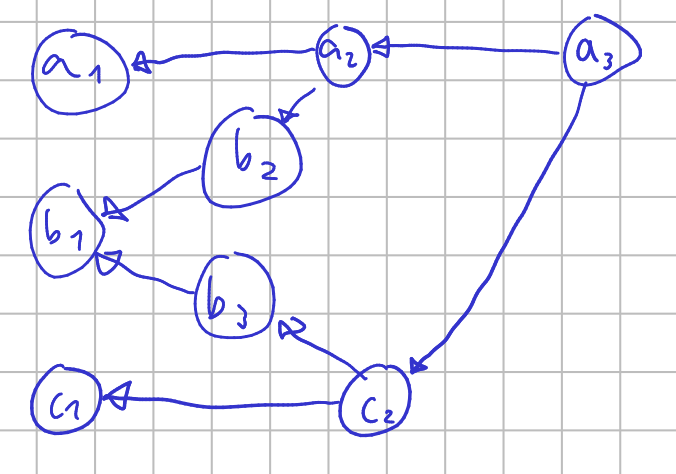
\includegraphics[width=.5\textwidth]{figures/fork_scenario_1.png}
%     \caption{An example scenario of a fork in a message graph, where $a_3$ could be considered invalid}
%     \label{fig:fork_scenario_1}
% \end{figure}
% \begin{figure}[h]
%     \centering
%     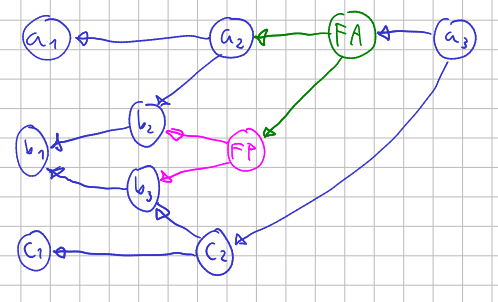
\includegraphics[width=.5\textwidth]{figures/fork_scenario_1_fixed.png}
%     \caption{The example message graph of Figure \ref{fig:fork_scenario_1} but where $a$ behaves correctly}
%     \label{fig:fork_scenario_1_fixed}
% \end{figure}
% Here is an invariant that arises naturally: for a message $M$, the induced subgraph of its dependencies only has forks that were acknowledged by author $M_\textit{author}$, i.e.




\section{Evaluation}
When evaluating our design, we focused on two metrics. The first was performance of the verification algorithm and the second was efficiency of storage.
Concerning performance, there are two things we are interested in: how is the scaling behaviour as we increase the number of messages we verify? and how do different optimizations affect the runtime?
Concerning storage, we compare how much less storage our design uses by storing account data in the message of a commit compared to storing the data in the tree and blob objects as in the delta-GOC-Ledger by Heisch \cite{delta-goc-ledger-heisch}.

\subsection{Methodology}
\subsubsection{Generating baseline Repository}
\label{sec:base-repo}
To get a baseline performance and storage measurement, we created a benchmark that contains random transactions between a fixed number of authors, where the number of transactions per author follows a heavy-tailed distribution (a Pareto-distribution in our case), as it often does in real-world scenarios \cite{bitcoin-distribution-transactions}. In the performance benchmark, the number of simulated transactions is varied to indicate asymptotic scaling of the runtime of different parts of the code. The number of authors is fixed at 10. Additionally there is an acknowledgement delay, meaning tokens that were given don't get acknowledged immediately. However the messages are assumed to always be replicated instantly, meaning all the participants know about the latest messages when creating a new one. Note that this doesn't mean that messages are totally ordered, since the immediate dependencies of an account message are only the relevant participants of a transaction.

\subsubsection{Generating Repository including Forks}
\todo{if there is time: specify a more general way to generate transaction data including forks and byzantine acknowledgements}

\subsubsection{Performance benchmark}
We generate repositories with the number of messages varying from 300 to 900 with a step size of 300.
To measure the runtime of different parts of the code, we use the \verb|perf_counter| function from the \verb|time| module in the standard library of python \cite{pythonPerfCounterNs}.
We split the code into various non-overlapping sections. Each section should either contain invariant checks directly or performance critical code.

\subsubsection{Storage Bench: Comparison of storage methods}
We take the simulation described in section \ref{sec:base-repo} and use it to create repositories with the same encoded transactions and the number of messages being 1000. The only difference between them is how the messages are stored and how many dependencies each message has.

In Method 1, the account data is stored as described in \ref{sec:syntax-of-msgs}. In Method 2, the account data is stored as nested tree and blob objects, as described in \cite{delta-goc-ledger-heisch}. More concretely json objects in our encoding map to tree objects and GOCs are represented as blob objects which contain the bytes that represent the number they store (using the functions \verb|int.to_bytes| and \verb|int.from_bytes| in the standard library of python to encode and decode respectively). \todo{if necessary: add figure that shows example of this visually.}

The number of dependencies is also varied. If we write ``with unnecessary dependencies'' we mean that a message stores a reference for each other author pointing to the last known message that the creator knew about, as opposed to just the last messages of the authors that appear in the transaction.

To measure the size of the generated repositories, we use the unix command \texttt{du} (disk usage) on the corresponding \texttt{.git} directory with the flag \texttt{-s} to get the total size this directory takes up. We also add the flag \texttt{--apparent-size} to get the size if each file occupied exactly the size on disk.

\subsubsection{Relevant Specs of System}
The Benchmarks are run on a Lenovo ThinkPad X13 2-in-1 with the specs shown in table \ref{tab:specs}.
One important thing to note when using WSL2 as a virtual machine is that the performance is degraded significantly when accessing files from a mounted directory \cite{wsl2FilesystemPerf}. We run the benchmark with associated data in the home directory, where this issue doesn't arise.
\begin{table}
\centering
\begin{tabular}{|l|p{6cm}|}
    \hline
    OS & WSL version 2.7.10.0 running Ubuntu 24.04.4 LTS with Microsoft Windows 11 Pro as host OS\\ \hline
    System Type & x64-based PC\\ \hline
    Processor & Intel(R) Core(TM) Ultra 5 125U, 1300 Mhz, 12 Cores, 14 Logical Processors\\ \hline
    Installed Physical Memory (RAM) & 16.0 GB\\ \hline
    Git version & 2.43.0 \\ \hline
\end{tabular}
\caption{relevant specs of the hard- and software used to perform benchmarks}
\label{tab:specs}
\end{table}

\subsection{Results}
\subsubsection{Performance of Verification Algorithm on baseline repository}
\begin{figure}
    \centering
    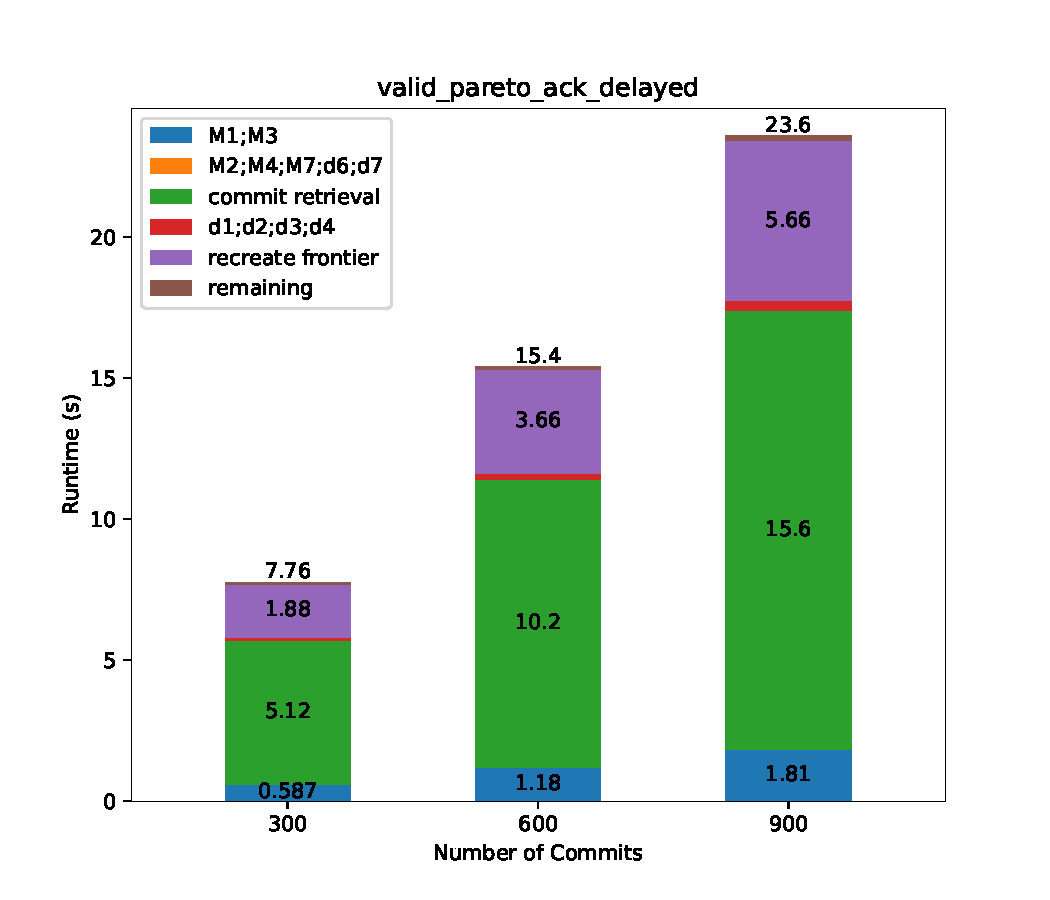
\includegraphics[page=1,width=.75\textwidth]{figures/valid_pareto_ack_delayed.pdf}
    \caption{Performance measurements on Bench 1}
    \label{fig:perf-result}
\end{figure}
\todo{add benchmark result without frontier caching optimization}
The results of the performance benchmark done on the baseline repository are shown in figure \ref{fig:perf-result}. The labels that are separated with semi-colons represent the code snippets responsible for checking the corresponding invariants. The part ``commit retrieval'' is the initial retrieval of the command line output by git and includes the checking of signatures. The part labelled ``remaining'' is the runtime that was not timed.
We see that the total running time (top of the bars) increases roughly linearly in the number of commits, however if we only take a look at the ``recreate frontier'' part, we can see that this part increases significantly more than linearly.

\paragraph{Discussion}
The reason ``recreate frontier'' is the biggest part of the time besides ``commit retrieval'', is because we use subprocesses to recreate the frontier, which happens in each commit. Although we try to limit the number of commits that are traversed (see section \ref{sec:impl-verification-alg}), there is still seems to be an inherent performance overhead with calling subprocess from python. The reason it scales quadratically is because the number of commits that maybe have to be traversed to recreate the frontier only increases during the runtime of the algorithm. If we get unlucky, we even have to traverse all of the commits in the causal history of the commit we are looking at (if none of the parents in the cache are parents of the commit).

\subsubsection{Storage Bench}
When measuring the size of the generated git repositories, we get the result shown in table \ref{tab:storage-res}. We see that our approach uses about 29\% of the space that Method 1 with unnecessary dependencies uses (proposed in \cite{delta-goc-ledger-heisch}) when looking at the effective space used on the disk and 37\% when looking at the apparent size of files.

We also see that the difference in effective space used doesn't change meaningfully when storing unnecessary dependencies in either case.
\begin{table}
    \begin{tabular}{|p{5cm}|l|l|}
        \hline
        \textbf{Method} & \textbf{Size on Disk} & \textbf{Apparent size}\\ \hline
        Method 1 with unnecessary dependencies & 18916 Kb & 1927 Kb\\\hline
        Method 1 & 18916 Kb & 1754 Kb\\ \hline
        Method 2 with unnecessary dependencies & 5428 Kb & 875 Kb\\ \hline
        Method 2 (ours) & 5424 Kb & 699 Kb\\ \hline
    \end{tabular}
    \caption{Result of storage benchmark}
    \label{tab:storage-res}
\end{table}
\paragraph{Discussion}
The difference in storage space between Method 1 and Method 2 can be attributed to our method not having to save so many additional objects and their references. Deduplication of GOCs is ineffective, because for each GOC we also have to store the blob identifier, which is a sha256 hash meaning that it takes up 32 bytes of space. Once the numbers stored in the blobs would get large enough for this to be worth it, collisions of such GOCs is so unlikely that practically no deduplication would happen.

The lack of a difference between effective space used when storing unnecessary dependencies can be attributed to the operating system reserving additional space for small files on the disk. Since many of our files are quite small, this results in space being available for storing the unnecessary dependencies without increasing the effective space used. We think that this would change in a real system where there would be a lot more than 10 participants involved, i.e. the size saved when only storing the necessary dependencies would be considerable.

\section{Related Work}
The design of the delta-GOC-Ledger, as well as of the 2P-BFT-Log was taken directly from the Masters Thesis of Heisch \cite{delta-goc-ledger-heisch} and the Paper of Lavoie \cite{2p-bft-log} respectively. What was attempted in this report was to unify the two designs. To do this, we took inspiration from the Blocklace paper by Almeida et al. \cite{blocklace-crdt}. Additionally, none of the papers mentioned above described a verification procedure, which we partly specified and implemented. We also extended the designs by limiting the number of dependencies per transaction and adding a new message type.

\section{Conclusion}
In this report, we explored how a verification algorithm of byzantine fault tolerant logs might look like. There is, however a lot that still has to be done; first of all, the problem of double spending still persists and has to be solved by designing a system that prevents correct replicas from losing tokens or tokens being created out of thin air. Additionally, the verification algorithm still has to be extended to include invariants F2 and F3, which should guarantee byzantine repellance, as defined in the Blocklace paper \cite{blocklace-crdt}.
The implementation of the verification algorithm can still be improved significantly by avoiding the subprocess-calls when recreating the frontier.
Furthermore, our implementation never clears commits out of the cache, because it always relies on them being present.
Our implementation is also memory bound. In order for the verification to be feasible, an incremental system would have to be developed, where memory can be offloaded to persistent storage efficiently.

\printbibliography

\end{document}